\section{Design}

Houdini is built using Python 3 and leverages a QEMU VM to provide a controlled testing environment for container security validation. Instead of running containers directly on the host system, Houdini spins up a dedicated VM, ensuring that any security vulnerabilities or container escapes remain isolated and do not affect the host system. This setup allows for highly reproducible security tests while minimizing unintended side effects on the underlying infrastructure.  

At the core of Houdini’s architecture, a Flask-based server runs on the host operating system (not inside the VM). This server acts as a bridge between the host and the QEMU virtual machine, facilitating communication between them. The Flask server is responsible for sending commands and configuration data to the guest VM and receiving trick execution results. When a trick is initiated, the **Houdini client on the host instructs the VM to start a new test. The VM then launches a container with the specified security configurations and executes the trick inside it.  

Once the trick completes, the VM collects the results and sends them back to the host via the Flask server. The host then processes this data, logs the results, and determines whether the container security mechanisms functioned as expected. This structured workflow ensures that Houdini remains independent of the host system’s container runtime while providing a reliable and repeatable environment for testing container confinement mechanisms.

\label{sec:design}

\subsection{Design Goals}

\houdini is designed to provide a systematic and reproducible approach to testing container confinement mechanisms. One of its primary goals is to evaluate whether container security features, such as namespaces, cgroups, seccomp, and Linux capabilities are effectively enforcing isolation. Many security tools rely on theoretical guarantees or static analysis, but Houdini focuses on empirical validation by executing controlled security tests, known as \enquote{tricks}, that verify the correct enforcement of security mechanisms. By doing so, \houdini ensures that container security mechanisms are correctly configured.

One of the goals of \houdini is not only for testing container isolation but also as a means to optimize container configurations. By systematically simulating various tasks within Docker containers, Houdini can help determine the minimal set of privileges required for a container to perform its intended function. For example, administrators can start with a container configured with broad privileges and then incrementally reduce permissions, such as Linux capabilities, seccomp filters, or resource limits, while monitoring task success. Houdini’s testing framework will identify the point at which functionality is maintained while unnecessary privileges are removed, thereby pinpointing the least privilege configuration that still allows the container to operate effectively. This approach is highly beneficial because it adheres to the principle of least privilege. Minimizing the privileges granted to a container reduces its attack surface, making it significantly harder for an attacker to exploit vulnerabilities.

The following are additional goals of Houdini:

\textbf{Verifying Whether Security Mechanisms Are Truly Working as Expected:}
Many security mechanisms in containerized environments, such as Linux namespaces, cgroups, seccomp filters, and capabilities—are intended to enforce process isolation and prevent privilege escalation. However, just because a security feature is enabled does not necessarily mean it is functioning correctly. Misconfigurations, improper runtime enforcement, and subtle implementation flaws can lead to unexpected security gaps. Houdini helps verify whether these security mechanisms are actually enforcing the intended restrictions by executing controlled tests (tricks) that attempt to bypass or manipulate confinement policies. If a test succeeds in breaking out of isolation, it provides direct evidence that the security mechanism is not functioning as expected.


\textbf{Identifying Gaps Between Intended Confinement Policies and Actual Enforcement:}
There is often a discrepancy between security policies that administrators configure and what is actually enforced at runtime. For example, a security policy may specify that a container should not have network access, but due to a misconfigured Docker setting, the container may still be able to establish outbound connections. Similarly, a container may be configured with resource constraints (e.g., CPU and memory limits via cgroups), but in practice, those constraints may be ineffective or bypassable. Houdini systematically tests these security policies against real execution environments to uncover where enforcement fails. By detecting these discrepancies, organizations can adjust their configurations and improve security postures, ensuring that containers remain properly confined under expected conditions.


\textbf{Challenging Misleading Security Assumptions with Empirical Testing:}
Container security is often discussed in terms of theoretical guarantees, with many security best practices based on assumptions rather than direct testing. For instance, documentation may state that a container running in unprivileged mode cannot escalate to root, but Houdini actively tests whether that is actually the case under different container configurations. By running real-world security validation instead of relying solely on security claims, Houdini helps challenge misleading assumptions and exposes where security mechanisms fail in practice. This is particularly important as container escapes and privilege escalation exploits continue to emerge, demonstrating that security controls do not always work as expected. By grounding security claims in measurable results rather than theory, Houdini helps researchers and practitioners develop more robust container security strategies.




In order to achieve the aforementioned goals, we designed \houdini with the following in mind:
\begin{dgenum}
  \item \label{dg:repro}\textit{Reproducible Results.} A key goal of \houdini is to ensure that tests yield consistent and repeatable results. By controlling system variables and maintaining a structured testing environment, Houdini allows researchers and practitioners to compare results across different system configurations and security policies.

  \item \label{dg:container}\textit{Separation from the Host.} \houdini is designed to run tests inside a controlled containerized environment within a virtual machine (VM), ensuring that even if a test triggers a security vulnerability, it does not compromise the host system running the tests. This design choice enhances the safety of security evaluations, preventing unintended side effects on the underlying infrastructure.

  \item \label{dg:test}\textit{Test Case Expressiveness.} \houdini test cases (called \enquote{tricks}) should be maximally expressive, such that some combination of steps can be used to achieve and test any desired result. It should be possible to define a new \houdini trick and modify existing tricks without modifying the \houdini binary. Moreover, it should be clear from reading a defined trick precisely what steps are involved, the consequences of each step passing or failing, and the overall nature of the exploit being tested.

  \item \label{dg:failures}\textit{Focus on Observing Failures, Not Preventing Them.} \houdini is built to identify security weaknesses rather than defend against attacks.
\end{dgenum}

\subsection{Security of the Testing Environment}

If Houdini were compromised during testing, it would not necessarily pose a threat to the host system due to the design of the testing environment. Houdini is intentionally designed to operate within a controlled, containerized environment inside a VM. This means that even if a test were to exploit a vulnerability within the containerized environment, the impact would be contained within the VM, isolated from the host system and other containers. The VM itself serves as an additional layer of security, providing a buffer that prevents the compromise from reaching the host infrastructure.

\subsection{Design of Tricks}

\begin{figure}
  \label{fig:state-machine}
  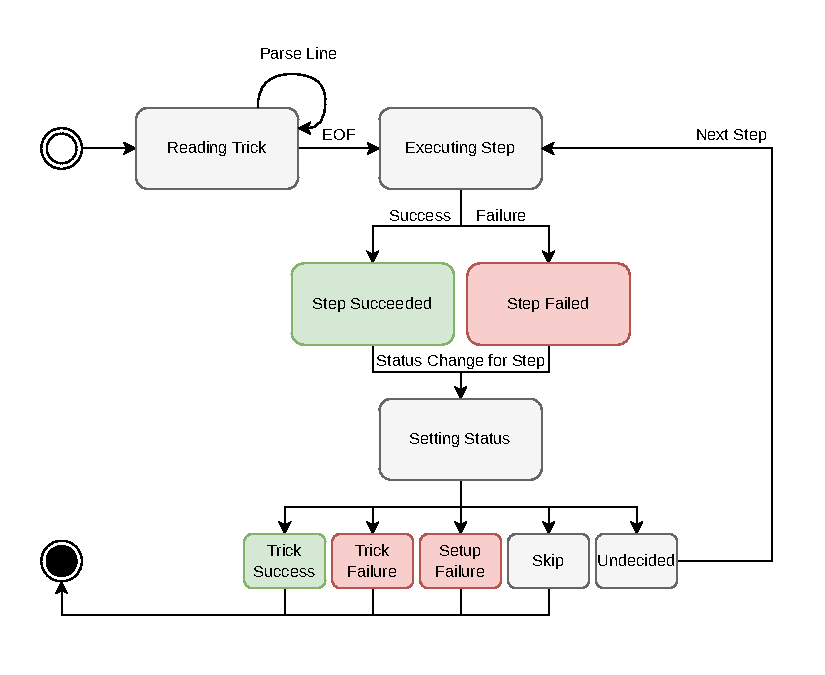
\includegraphics[width=1\linewidth]{figs/houdini-state-machine.pdf}
  \caption{A state machine diagram of Houdini running a Trick.}
\end{figure}

In containerized environments, security challenges often arise from vulnerabilities within specific components of the architecture. As such, understanding the relationships between the different components—such as container registries, images, runtime, namespaces, cgroups, and various security modules like eBPF, seccomp, and Linux capabilities—is crucial for identifying potential attack surfaces. This is where a comprehensive architecture diagram comes into play.

\begin{figure}
  \label{fig:architecture}
  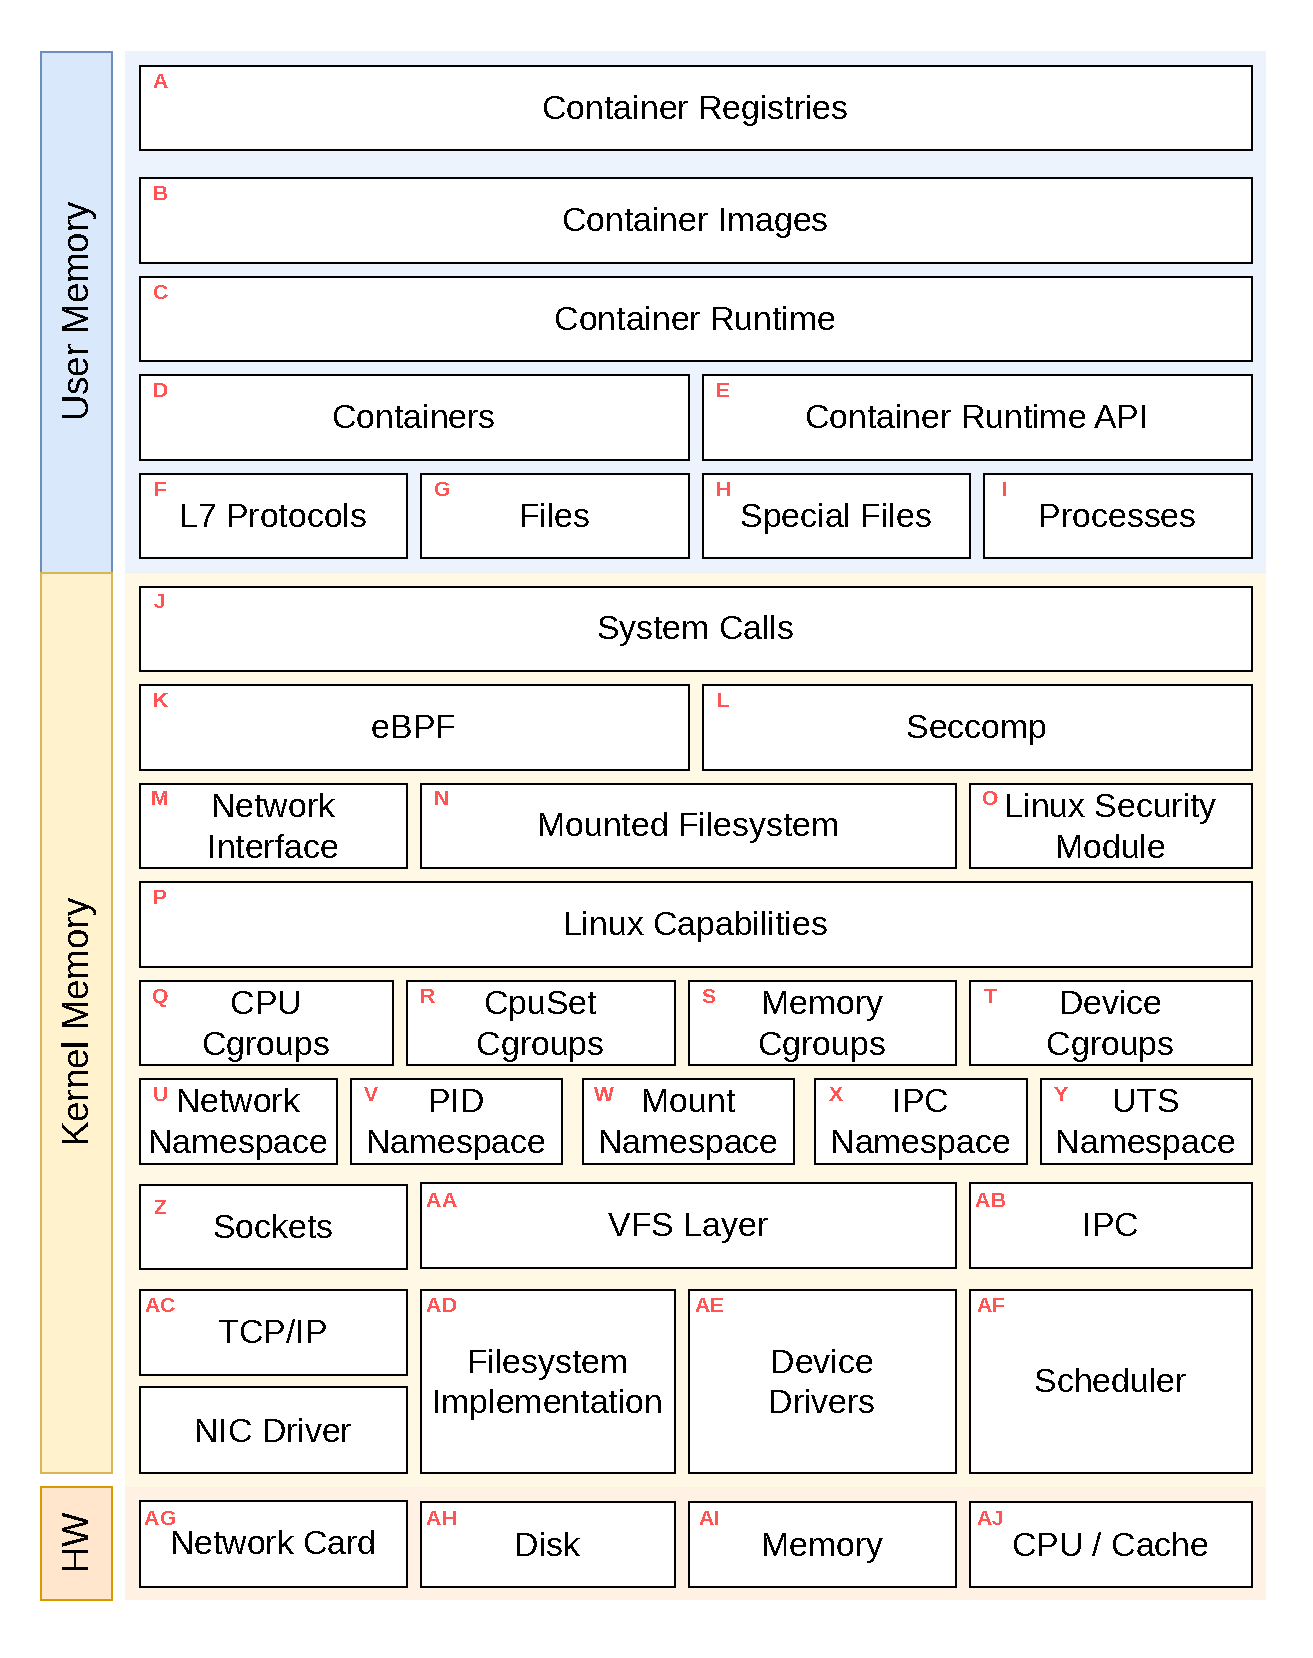
\includegraphics[width=1\linewidth]{figs/exploit-coverage.pdf}
  \caption{An architectural diagram of a container deployment environment depicting the attack surface created by its various components.}
\end{figure}

Figure 2 outlines the key components of a containerized system, highlighting the critical paths and interactions that security tests should focus on. Security testing should aim to cover these components extensively to ensure that vulnerabilities in any of these layers are adequately addressed. However, some components, like network interfaces, system calls, and cgroups, are more frequently targeted in real-world attacks and thus warrant more attention in testing. The diagram will guide our understanding of which components to prioritize during testing, ensuring that our coverage is both thorough and effective.
